\clearpage
\twocolumn
\section{Frontier: Large-Structure Maintenance Diagnostics}
\label{sec:frontier}
\paragraph{Version and scope.}
Frontier-1 is a separate public-development protocol, not a replacement
for frozen v2 or Challenge-2. Six original objects contain 1,509 placed
parts and instantiate eight contracts each, yielding 48 tasks.
The 117,910 historical conditions are not counted as Frontier tasks.
Its nominal geometry extends the envelope to 512 parts, integer origins
0--95 and bodies in $[0,96]^3$, while retaining the same rectangular
catalog and vertical action semantics. No arbitrary CAD connectors,
force balance, robot motion, or image-only results are claimed.

\begin{figure*}[t]
\centering
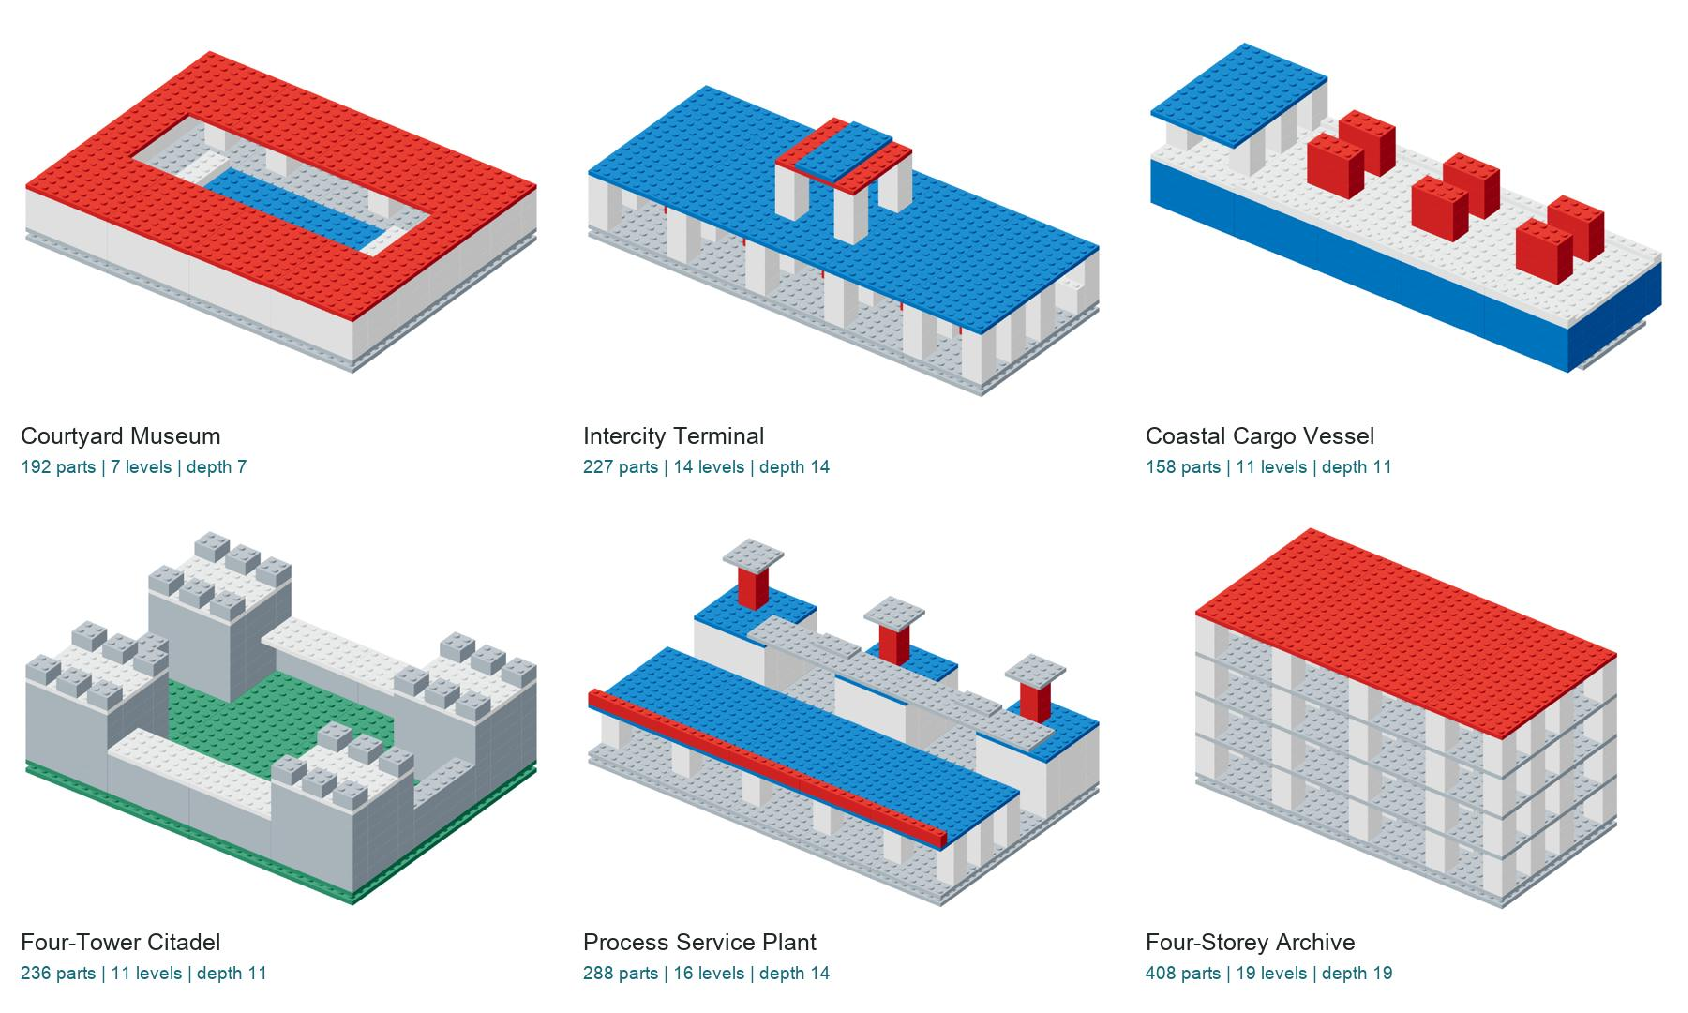
\includegraphics[width=\textwidth]{figures/frontier-models.pdf}
\caption{All six Frontier objects, without selection. Functional colors,
deep footprints, hollow towers, service galleries and stacked floors
replace the previous four-stud-deep challenge strips. Greater part count
is not itself evidence of greater reasoning difficulty.}
\end{figure*}

\begin{table}[t]
\centering\small
\begin{tabular}{lrrrr}
\toprule Object & Parts & Levels & Depth & $X\times Z$\\\midrule
\tableinput{tables/frontier-models.tex}
\bottomrule
\end{tabular}
\caption{Levels count distinct bottom-$Y$ coordinates. Depth is the
longest all-lower-overlap precedence chain, not a learned difficulty score.}
\end{table}

\subsection{Related-Work Audit and Bounded Opportunity}
Generation and larger objects are not novel by themselves:
BrickNet~\cite{kulits2026bricknet} supplies much richer human-designed
LDraw content and arbitrary connector semantics; BrickGPT~\cite{pun2025brickgpt}
includes physics-aware rollback; BrECS~\cite{ahn2024brecs} already
considers part budgets and types. MEPNet~\cite{wang2022manual} handles
unseen composed parts and symmetry; TreeSBA~\cite{guo2024treesba}
predicts assembly from multiple views. BC-Bench~\cite{liu2026composer}
directly measures brick selection and pose.

LEGO-Puzzles~\cite{tang2025legopuzzles} includes multi-step spatial
reasoning and, in its revised submission, a 1--8-step planning set.
PhyBlock~\cite{ma2025phyblock} includes 400 assembly tasks, 2,200 VQA
tasks, progressive levels, diagnosis, robustness and counterfactuals.
LEGO Co-builder~\cite{huang2025cobuilder} studies fine-grained instruction,
object and state detection. Break and Make~\cite{walsman2022break}
already couples inspection, disassembly and rebuilding.
WorkBenchMark~\cite{ma2026workbenchmark} provides 400 Duplo tasks,
four tiers and robot/VLA evaluation; Eye-in-Finger~\cite{tang2025eyefinger}
addresses occlusion and precise physical error correction.

Thus neither ``repair'', ``active inspection'', ``multiple tasks'',
nor ``long-horizon assembly'' establishes novelty. Our bounded
opportunity is a shared-object diagnostic contract tying minimum
intervention certificates, executable maintenance, finite-world
uncertainty and explicit resource costs together. This combination
is less directly covered in the reviewed protocols; we do not prove
absence across all literature or claim a first-ever capability.
The Chinese report records primary links, scope and overlaps.

\subsection{Eight Executable Contracts}
\paragraph{Minimum-action service.}
Input is a current assembly, full target and service ID.
Actions remove a current ID or place that target inventory part at its
target pose. No in-place recoloring or group moves are allowed.
A legal trace must restore all target parts within the declared budget.
Let $C$ be the transitive closure of overhead footprint overlaps
starting from service IDs. Every member of $C$ must be removed and
replaced, so $2|C|$ is a lower bound. Reverse-height removal followed
by height-ordered placement achieves it in these cases, establishing
10--50-action optimal witnesses. This is polynomial closure reasoning,
not evidence of general search hardness.
Report legal prefix, final exactness, action count, lower bound and excess.

\paragraph{Access certificate.}
Return exactly $C$, including service IDs, and any legal removal order.
The evaluator checks minimum-set equality and executes the supplied order.
An independent upward-graph traversal verifies closure. The IDs removed
by the service solver must equal the certificate, providing a same-object
cross-task consistency control.

\paragraph{Parallel schedule.}
Return synchronous batches with at most four abstract workers.
Every lower footprint-overlapping part is a prerequisite and must
occur in an earlier batch. IDs must occur exactly once; all must finish.
Report coverage, makespan and the workload lower bound $\lceil n/4\rceil$.
This conservative all-prerequisite contract is stronger than the
one-stud-support predicate. Optimality and simultaneous robot motions
are not claimed. A serial height-order baseline succeeds, but takes
$n$ rounds; success alone does not reward efficiency.

\paragraph{Minimum support intervention.}
Choose a minimum-cardinality subset of a public candidate set whose
forced simultaneous deletion eventually removes the stated goal under
iterative zero-direct-support propagation. Report forced IDs and the
entire propagated set, including those IDs. Enumerating the candidate
power set establishes optimal cardinality; any optimal choice is accepted.
Forced deletion ignores access. This measures a graph/geometry
counterfactual, not physical collapse.

\paragraph{Inventory-constrained replacement.}
Replace an $8\times4$ plate using a limited mixed inventory of smaller
plates. Local cells must be covered exactly once, without protrusion.
The sum of the largest available plate areas yields a cardinality
lower bound. Each released instance has a feasible tiling attaining it;
an independent public-input exact-cover search verifies a witness.
Alternative optimal tilings are accepted. The equivalence is occupied
slab volume, not unchanged seams, contacts or BOM. These small local
problems are calibration tasks, not general semantic redesign.

\paragraph{Admissible hidden topology.}
Three foundation slabs each admit two four-brick tilings: two pairs of
lengthwise plates or four crosswise plates. Their Cartesian product
gives eight worlds with equal colored occupied cells and BOM but
different seams. Geometry outside the slots, the finite grammar and
one slot observation are public. Return all four compatible world IDs.
Guessing one private reference is false certainty. Every world is
geometry-validated; occupancy equality is not a claim of identical
RGB seam pixels. There is no seam RGB input in this track.

\paragraph{Budgeted contingent inspection.}
The same eight hidden worlds are identified by a query decision tree.
Three local queries cost 1, 2 and 3; a full query costs 9.
At each internal node, the simulator returns that query's symbolic
value for the current world; the branch determines the next node.
Every world must reach its correct leaf with worst-case cost at most 6.
Repeated queries, unknown queries, missing branches and incorrect leaves
fail. Report world coverage and worst-case cost. A minimax public-input
solver selects queries; no real camera or robot interface is asserted.

\paragraph{Distributed mixed-fault patch.}
Three regions contain translation, quarter-turn and color faults.
The full current and target structures are public. Return exact faulty
current IDs and only their replacement part records. Unlisted geometry
is preserved, and the reconstructed result must exactly match up to
per-part yaw symmetry. The patch is not a physical action trace.
This is a transparent diagnostic calibration, not hard perception.

\subsection{Baselines, Disclosure and Limits}
\begin{table}[t]
\centering\small
\begin{tabular}{lrr}
\toprule Task & Public solver & Shortcut\\\midrule
\tableinput{tables/frontier-baselines.tex}
\bottomrule
\end{tabular}
\caption{Actual deterministic algorithm runs, six source objects per
task. No paid inference or learned-model results. Solvers receive only
exported public fields. Shortcut definitions and per-case receipts are
released; serial scheduling is valid but slower.}
\end{table}

The public solvers use graph traversal, exhaustive candidate deletion,
first-uncovered-cell tiling search, direct reference comparison and
minimax query trees. The evaluator and solver do not share target
answer objects. Forty-eight positive and forty-eight constructed negative
controls separate correctly. These are validator checks, not 96 model
predictions. Tests cover schema coercion, coordinate bounds, legal action
order, omitted/duplicated steps, alternative tilings, query budgets,
all-world coverage and independent cell-map support.

All 48 new tasks are symbolic or finite-observation contracts. Four-view,
layer and exploded images are reviewer assets, not undeclared model
observations. Existing Challenge visual contracts remain separate.
Within a track, models receive identical public JSON and budgets;
raw and harness-assisted outputs must be reported separately.
Use source-grouped statistics on six objects, not 48 independent samples.
Model inference, human calibration and externally reproduced results
remain unmeasured. Public development data are not contamination-resistant
confirmation data. Reference checking and larger scenes do not justify
raising empirical discrimination or application-validity claims.
